% Comandi d'intestazione, formato pagina, lingua
\documentclass[12pt,a4paper]{article}
\usepackage[utf8]{inputenc}

\setlength{\parindent}{0pt}
% \usepackage[italian]{babel} % bibliografia
% Formato pagina "truccato" (by giuliof)
\usepackage[left=2cm,right=2cm,top=2.5cm,bottom=2.5cm]{geometry}
% Colonne
%~ \usepackage{multicol}
% Numerelli nel tondino (Wingdings-style)
%~ \usepackage{pifont}

% Palatino font
\renewcommand*\rmdefault{ppl}

%Non porre le immagini sotto le note a piè di pagina
% \usepackage[bottom]{footmisc}

%%% Pacchetti per l'ambiente matematico:
% pacchetto standard, fonts extra, simboli extra
\usepackage{amsmath}
\usepackage{amsfonts}
\usepackage{amssymb}

%%% Pacchetti di grafica
\usepackage{graphicx}
\usepackage{float}  % per tabelle non flottanti
\usepackage{adjustbox}
\usepackage{tikz}
\usepackage{forest,array}
\usetikzlibrary{shadows}

\forestset{
  giombatree/.style={
  for tree={
    grow = east,
    parent anchor=east,
    child anchor=west,
    edge={rounded corners=2mm},
    fill=violet!5,
    drop shadow,
    l sep=10mm,
    edge path={
      \noexpand\path [draw, \forestoption{edge}] (!u.parent anchor) -- +(5mm,0) -- (.child anchor)\forestoption{edge label};
    }
  }
}
}

\usepackage[hidelinks]{hyperref} % Nasconde link dall'indice

% Item label (pallino pieno, vuoto, trattino)
\renewcommand{\labelitemi}{$\bullet$}
\renewcommand{\labelitemii}{$\circ$}
\renewcommand{\labelitemiii}{--}

% PDF page in landscape
\usepackage{pdflscape}

%~ Bibliografia e citazioni
\usepackage[style=numeric,backend=bibtex]{biblatex}

\addbibresource{bibliografia.bib}

\setcounter{section}{-1}
\setcounter{secnumdepth}{4}

\title{Appunti di Sistemi Operativi}
\author{\texttt{<giomba@live.it>}}
\date{}

\begin{document}

\maketitle
\tableofcontents

\clearpage

\section{Introduzione}
\subsection{Informazioni generali}
Questi appunti, tratti dalle lezioni in aula del prof. Marco~Avvenuti,
sono da intendersi come appunti riassuntivi.

Questi appunti \textit{non} sono stati revisionati dal prof. Marco~Avvenuti.
I testi ufficiali a cui fare riferimento per lo studio di questa
disciplina sono elencati nella bibliografia.

Questi appunti potrebbero essere utili per il superamento dell'esame di
Sistemi Operativi del corso di laurea triennale di Ingegneria Informatica,
ma questo non implica che siano affidabili.

L'autore non si assume nessuna responsabilità sull'uso proprio,
e specialmente improprio, che si vorrà fare di questi appunti.

\subsection{Informazioni particolari}
Questi appunti sono stati scritti, raccolti, ampliati e ricomposti da:
\begin{itemize}
  \item giomba \texttt{<giomba@live.it>}
\end{itemize}
che ha fatto uso anche degli appunti di:
\begin{itemize}
  \item F. Barbarulo \small{\texttt{<info@notestack.it>}}
  \item alex.sieni
\end{itemize}

Questi appunti sono abbastanza schematici; per una spiegazione esaustiva
fare riferimento al testo ufficiale; per una spiegazione più dettagliata
di questa, ma meno dettagliata del libro, fare riferimento agli appunti
di F. Barbarulo.

Questi appunti non sono completi: facendo riferimento al testo principale
\cite{ancilotti:so}, è assente il capitolo sulla protezione, mentre il
capitolo su Unix è solo accennato; ma c'è una buona notizia.

Il codice sorgente di questi appunti è stato versionato con git e viene
rilasciato gratuitamente sotto licenza GPL3: può essere consultato
facendo esplicita richiesta all'autore, che invita a ampliare, correggere
e terminare il lavoro da lui incompiuto.

\subsection{Cinque}
Non ve ne importa niente, ma in corrispondenza col superamento dell'esame
di Sistemi~Operativi, della scrittura finale di questa sezione e del
rilascio definitivo di questi appunti in data 9~gennaio~2018, è morto
il mio professore di italiano e latino del liceo.

Lui era un professore speciale, più umano della media, a tratti quasi un
amico, che sapeva ampliare il rapporto professionale con gli studenti
con qualcosa che dava una marcia in più nella crescita professionale e umana
dell'individuo, qualcosa che andava di là dagli schemi tradizionali
dell'insegnamento.

È merito suo se ho imparato \emph{rosa, rosae, rosae, rosam, rosa, rosa},
ma anche se so che il fandango è un tipo di ballo spagnolo, se riesco
a leggere il significato nascosto di Stand~By~Me\footnote{Rob Reiner},
se ancora oggi chiamo i miei vecchi compagni del liceo.

O capitano, mio capitano!

Requiescat.

\clearpage

\begin{landscape}
\section{Mappe}
\subsection{Argomenti generali}
\begin{center}
\begin{forest} giombatree,
[ Argomenti Generali
  [ Tassonomia di Flynn
    [ SISD ]
    [ SIMD ]
    [ MISD ]
    [ MIMD
      [ SM ]
      [ DM ]
    ]
  ]
  [ Processi
    [ Stato dei processi]
    [ Sostituzione del codice]
    [ Primitive
      [fork]
      [exec]
      [exit]
      [wait]
    ]
  ]
]
\end{forest}
\end{center}
\end{landscape}

\section{Tassonomia di Flynn}
\subsection{Terminologia utilizzata}
\begin{itemize}
  \item Instruction Processor (IP): elemento che esegue istruzioni
  \item Data Processor (DP): elemento che elabora dati
  \item Instruction Stream: flusso di istruzioni eseguite da un IP
  \item Data Stream: flusso di dati che vengono elaborati da un DP
  \item Instruction Memory (IM): contiene istruzioni
  \item Data memory (DM): contiene dati
\end{itemize}

Le memorie vengono rappresentate con una forma triangolare per evidenziare
la presenza di una gerarchia \cite[25]{ancilotti:so}.

I flussi si distinguono in:
\begin{itemize}
  \item \emph{single stream}: è possibile identificare un unico flusso
  \item \emph{multiple stream}: è possibile identificare più flussi
\end{itemize}

Le macchine possono essere inserite in quattro categorie:

\begin{tabular}{| c | c | c |}
\hline
    & SD    & MD    \\  \hline
SI  & SISD \adjustimage{width=3cm,padding=.1cm,valign=m}{img/flynn/sisd.png}  & SIMD \adjustimage{width=3cm,padding=.1cm,valign=m}{img/flynn/simd.png} \\  \hline
MI  & MISD                                                  & MIMD \adjustimage{width=3cm,padding=.1cm,valign=m}{img/flynn/mimddm.png} \adjustimage{width=3cm,padding=.1cm,valign=m}{img/flynn/mimdsm.png} \\  \hline
\end{tabular}

\subsection{SISD - Single instruction and single data streams}

\centerline{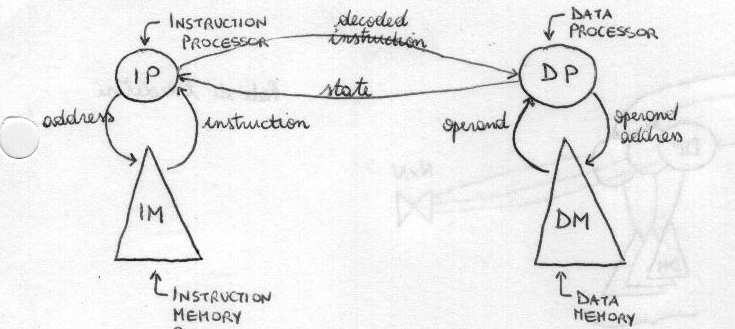
\includegraphics[width=10cm]{img/flynn/sisd.png}}

La macchine in grado di eseguire un solo flusso di istruzioni possono
comunque essere multiprogrammate, e i processi che vengono eseguiti sono
detti \emph{processi concorrenti} in quanto \emph{concorrono} per l'utilizzo
dell'unica unità di elaborazione disponibile.

Esempio: il computer monoprocessore di P. Corsini
\begin{itemize}
  \item parte controllo (IP);
  \item parte operativa (DP);
  \item registro di stato (FLAG);
  \item memoria (IM + DM)
\end{itemize}

\subsection{MISD - Multiple instruction stream and single data stream}

Non esistono macchine di questo tipo, sono un puro esercizio di stile.

Taluni ritengono macchine MISD le macchine dotate di
pipeline \cite[209]{frosini:architetturacalcolatori},
in cui più istruzioni entrano nella pipeline,
e attività diverse del ciclo macchina\footnote{fetch, decode, read, execute, write}
necessario ad eseguirle, vengono effettuate parallelamente.

\subsection{SIMD - Single instruction stream and multiple data stream}

\centerline{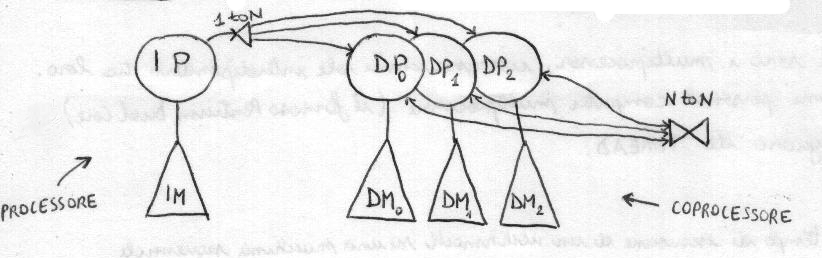
\includegraphics[width=10cm]{img/flynn/simd.png}}

Si tratta di macchine dedicate che eseguono task CPU-bound.
Tutti i coprocessori presenti eseguono la stessa operazione, ma su sottoinsiemi
di dati differenti.

Ad esempio, le macchine SIMD possono lavorare in parallelo su piccole parti
di una matrice più grande, sfruttandone le proprietà matematiche.

\subsection{MIMD - Multiple instruction and multiple data streams}

Le macchine MIMD possono essere ulteriormente suddivise in:
\subsubsection{DM - Distributed memory}
\centerline{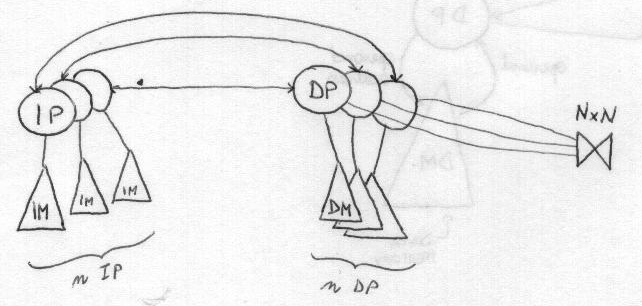
\includegraphics[width=10cm]{img/flynn/mimddm.png}}
Macchine MIMD di tipo DM non sono altro che più macchine SISD collegate
tra loro con una qualunque rete (es. Internet).

Le "singole" macchine SISD che compongono la macchina MIMD sono autosufficienti
e del tutto indipendenti tra loro; il guasto di una macchina SISD non
pregiudica il funzionamento del sistema (entro determinati limiti).

\subsubsection{SM - Shared memory}
\centerline{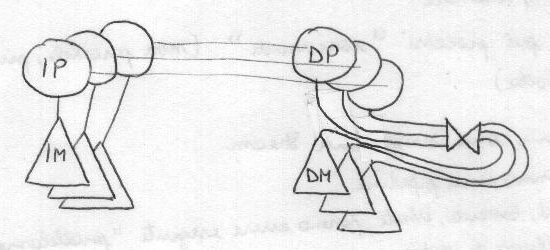
\includegraphics[width=10cm]{img/flynn/mimdsm.png}}
Macchine MIMD di tipo SM sono macchine multiprocessore.
Tutta la memoria è condivisa e viene vista come un'unica memoria, e viene
resa accessibile a qualunque DP.

Le macchine MIMD di tipo SM multiprogrammate eseguono processi detti
\emph{processi paralleli}, in quanto vengono eseguiti \emph{parallelamente}
sulle diverse unità di elaborazione.

A differenza delle macchine MIMD DM, le macchine MIMD SM non possono
tollerare guasti ad una delle loro unità, in quanto interdipendenti tra loro.

\section{Speed-Up}
  $$ S = \frac{T_1}{T_N} < N $$

  dove

  \begin{itemize}
    \item benchmark è un insieme di task da eseguire;
    \item $ T_1 $ è il tempo di esecuzione di un determinato benchmark su
      una macchina monoprocessore;
    \item $ T_N $ è il tempo di esecuzione dello stesso benchmark su
      una macchina multiprocessore con N processori
  \end{itemize}

  In un mondo ideale, $ S = N $.

  Tuttavia vi sono sempre alcuni task che non possono essere che eseguiti
  sequenzialmente (non sono parallelizzabili), che abbassano lo speedup.
  Per tenere conto di questi task, si può utilizzare una definizione più
  esaustiva dello speedup, dato dalla legge di Amdahl.

  Legge di Amdahl
  $$ S = \frac{T_1}{T_{seq} + (\frac{T_1 - T_{seq}}{N})} < \frac{T_1}{T_{seq}} $$

\section{Reti di interconnessione}
Terminologia utilizzata:

\begin{itemize}
  \item \emph{Diametro}: massimo numero di hop necessario per far comunicare due host
  \item \emph{Partizionamento}: suddivisione di una singola rete in più sottoreti indipendenti
\end{itemize}

Tabella riassuntiva:

\begin{tabular}{| l | p{2cm} | p{2.5cm} | p{2cm} | c | c |}
\hline
Tipo            & Esempio & Collegamenti per nodo & Points of Failure   & Diametro            & Scalabilità       \\ \hline
Bus             & \adjustimage{width=2cm,padding=.1cm,valign=m}{img/net/bus.png}          & 1                     & 1                   & --                  & no ($ N << 100 $) \\ \hline
Point to Point  & \adjustimage{width=2cm,padding=.1cm,valign=m}{img/net/point2point.png}  & 2                     & 1                   & N - 1               & sì                \\ \hline
Ring            & \adjustimage{width=2cm,padding=.1cm,valign=m}{img/net/ring.png}         & 2                     & 2                   & $ \frac{N}{2} $     & sì                \\ \hline
Mesh            & \adjustimage{width=2cm,padding=.1cm,valign=m}{img/net/mesh.png}         & $ >2 $ (es 4)         & --                  & $ 2(\sqrt{N} - 1) $ & sì                \\ \hline
Mesh toroidale  & \adjustimage{width=2cm,padding=.1cm,valign=m}{img/net/mesh-toroid.png}  & $ >2 $ (es 4)         & --                  & $ \sqrt{N} $        & sì                \\ \hline
Tree            & \adjustimage{width=2cm,padding=.1cm,valign=m}{img/net/tree.png}         & $ >2 $ (es 3)         & 1                   & $ 2 log(N) $        & sì                \\ \hline
\end{tabular}

Alcune considerazioni:

\begin{itemize}
  \item Il bus può essere pilotato da un solo dispositivo alla volta, detto master, in mutua esclusione;
  \item Nelle reti punto-punto, i nodi intermedi devono occuparsi anche delle connessioni dei nodi periferici;
  \item Negli alberi, la rottura di un collegamento è tanto più dannosa quanto più è vicino alla radice;
  \item Negli alberi, un collegamento è tanto più trafficato quanto più è vicino alla radice.
\end{itemize}

\section{Schedulazione}
Un sistema di schedulazione è caratterizzato dai seguenti parametri:
\begin{itemize}
  \item \textbf{utilizzazione della CPU}: percentuale di uso proficuo
    della CPU per unità di tempo;
  \item \textbf{turnaround time}: tempo medio di completamento di un
    processo, dall'istante in cui entra in coda pronti, all'istante in
    cui termina;
  \item \textbf{throughput rate}: numero medio di processi completati
    per unità di tempo; è l'inverso del \textit{turnaround time};
\end{itemize}

Per ogni processo è possibile calcolare i seguenti valori:
\begin{itemize}
  \item \textbf{tempo di risposta}: intervallo temporale che intercorre
    tra l'ingresso di un processo in coda pronti, alla sua terminazione;
  \item \textbf{tempo di attesa}: intervallo temporale che intercorre
    tra l'ingresso di un processo in coda pronti, e l'inizio della sua
    esecuzione;
\end{itemize}

\begin{center}
\begin{forest} giombatree,
[ Schedulazione
  [ General purpose
    [ con prelazione
      [ SRTF ]
      [ RR ]
    ]
    [ senza prelazione
      [ FCFS ]
      [ SJF ]
    ]
  ]
  [ Realtime
    [ RM ]
    [ EDF ]
  ]
  [ Code Multiple ]
]
\end{forest}
\end{center}

\paragraph{Condizione sufficiente} per schedulabilità di $n$ processi con Rate Monotonic
$$ U \leq n(2^{\frac{1}{n}} - 1) $$

\section{Sincronizzazione tra processi}
\begin{center}
\begin{forest} giombatree,
[ Interazione
  [ Tipi
    [ Competizione ]
    [ Collaborazione ]
    [ Interferenza ]
  ]
  [ Modelli
    [ Ambiente globale ]
    [ Ambiente locale ]
  ]
]
\end{forest}
\begin{forest} giombatree,
[ Sincronizzazione
  [ Problemi
    [ Mutua Esclusione ]
    [ Buffer limitato / Produttore-Consumatore ]
    [ Lettori-Scrittori ]
    [ 5 filosofi ]
  ]
  [ Soluzioni
    [ Test-and-Set-Lock
      [ lock(); unlock() ]
    ]
    [ Semafori
      [ wait(); signal() ]
    ]
    [ Monitor e variabili condition ]
    [ send(); receive() ]
  ]
]
\end{forest}
\begin{forest}
[ Deadlock
  [ Cause
    [ Mutua esclusione ]
    [ Hold and Wait ]
    [ No preemption ]
    [ Circular wait ]
  ]
]
\end{forest}
\end{center}

\subsection{Problemi}
\subsubsection{Problema del buffer limitato}
\subsubsection{Problema dei lettori-scrittori}
\subsubsection{Problema dei 5 filosofi}

\subsection{Soluzioni ai problemi di mutua esclusione e comunicazione}
\subsubsection{Test and Set Lock}
\paragraph{Uso di Test and Set Lock}
\begin{verbatim}
  ···
  lock();
  ··· sezione critica ···
  unlock();
  ···
\end{verbatim}

\paragraph{Implementazione di Test and Set Lock}
\begin{verbatim}
lock:
  TSL x, %reg
  CMP $1, %reg
  JE lock
  RTS

unlock:
  ST $1, x
  RTS
\end{verbatim}

\subsubsection{Semafori: wait(); signal()}
\paragraph{Uso dei semafori}
\subparagraph{Per la mutua esclusione}
\begin{verbatim}
  ···
  wait(semaforo);
  ··· sezione critica ···
  signal(semaforo);
  ···
\end{verbatim}

\subparagraph{Per la sincronizzazione}
\begin{verbatim}
  consumatore:
    ···
    wait(disponibile);
    ··· consuma ···
    signal(consumato);
    ···

  produttore:
    ···
    wait(consumato);
    ··· produci ···
    signal(disponibile);
    ···
\end{verbatim}

\paragraph{Implementazione di semafori}
\begin{verbatim}
struct Semaphore {
  int value;
  PCB queue;  /* PCB = Process Control Block struct */
} s;

wait(Semaphore s) {
  if (svalue == 0) {
    < blocca processo su s.queue >
  }
  else {
    --s.value;
  }
}

signal(Semaphore s) {
  if ( < ci sono processi bloccati su s.queue > ) {
    < estrae e sblocca un processo >
  }
  else {
    ++s.value;
  }
}
\end{verbatim}

\subsubsection{Monitor e variabili condition}
L'uso dei semafori fa affidamento sull'assenza di errori del programmatore
utente e sulla sua onestà e buonsenso. È necessario introdurre dei costrutti
sintattici a più alto livello per evitare situazioni spiacevoli: i \emph{monitor}
e \emph{le variabili condition}. \cite[223]{silberschatz:osc}

\paragraph{Uso di un monitor}
Il monitor garantisce che un solo processo alla volta possa eseguire le
funzioni definite al suo interno.

\begin{verbatim}
monitor un_nome {
  ··· shared variables ···
  function F1(···) {
    ···
  }
  function Fn(···) {
    ···
  }
  init_code(···) {
    ···
  }
}
\end{verbatim}

\paragraph{Uso di variabili condition}
I processi usano le variabili condition per bloccarsi in attesa di un segnale
da un altro processo.

Dichiarazione di una variabile condition:
\begin{verbatim}
  condition x;
\end{verbatim}

Attesa su una variabile: la \texttt{wait} è sempre bloccante.
\begin{verbatim}
  x.wait();
\end{verbatim}

Notifica a un processo in attesa: la \texttt{signal} risveglia
un processo (se ce n'è uno in coda), altrimenti non fa niente.
\begin{verbatim}
  x.signal();
\end{verbatim}

Quando si notifica ad un processo che può continuare la sua esecuzione,
possiamo adottare due politiche:
\begin{itemize}
  \item \textbf{signal and wait} risveglia il processo bloccato e mette
    in attesa il processo che esegue la signal;
  \item \textbf{signal and continue} risveglia il processo bloccato, ma,
    il processo che esegue la signal, prima di cedergli l'esecuzione,
    finisce di fare le sue operazioni;
\end{itemize}

\paragraph{Implementazione di un monitor tramite semafori}
\subparagraph{Codice di inizializzazione}
\begin{verbatim}
  x_count = 0;
  x_sem.value = 0;
\end{verbatim}

\subparagraph{Monitor}
\begin{verbatim}
  wait(mutex);
  ··· corpo della procedura ···
  if (next_count > 0) {
    signal(next);
  }
  else {
    signal(mutex);
  }
\end{verbatim}

\subparagraph{Variabili condition}
\begin{verbatim}
  x.wait():
    x_count++;
    if (next_count > 0) {
      signal(next);
    }
    else {
      signal(mutex);
    }
    wait(x_sem);
    x_count--;

  x.signal():
    if (x_count > 0) {
      next_count++;
      signal(x_sem);
      wait(next);
      next_count--;
    }
\end{verbatim}

\subsection{Deadlock (stallo)}

Condizioni necessarie (ma non sufficienti) per il deadlock con risorse in
unica istanza.

\begin{itemize}
  \item mutua esclusione  (mutual exclusion)
  \item possesso e attesa (hold and wait)
  \item assenza di revoca
\end{itemize}

Condizione sufficiente:

\begin{itemize}
  \item attesa ciclica (circular wait)
\end{itemize}

Nel caso in cui le risorse siano presenti in più istanze, l'attesa ciclica
viene declassata a condizione necessaria.

\subsubsection{Prevenzione statica}
Consiste nell'impedire, in fase di compilazione, che si verifichi una delle
condizioni necessarie. Queste tecniche non sono efficienti, perché contraddicono
la buona norma modulare del sistema.

\begin{itemize}
  \item \textbf{Possesso e attesa} Per risolverla, si impedisce ai
  processi di fare richieste di risorse annidate tra loro, oppure si
  obbliga un processo a richiedere le risorse di cui ha bisogno tutte
  contemporaneamente prima di iniziare la sua esecuzione.

  \item \textbf{Assenza di revoca} Per risolverla, si permette al
  sistema di revocare le risorse già assegnate ad un processo, e di
  farlo ripartire solo quando saranno nuovamente disponibili sia la
  nuova che ha chiesto sia tutte quelle che aveva anche prima della
  revoca.

  \item \textbf{Attesa circolare} Per risolverla, si associa un numero
  d'ordine a ogni risorsa. Le risorse vengono assegnate ai processi in
  ordine crescente. Un processo non può richiedere una risorsa con
  numero d'ordine inferiore ad una risorsa che gli è già stata
  assegnata.
\end{itemize}

\subsubsection{Prevenzione dinamica}
\paragraph{Algoritmo del banchiere}
Lo stato del sistema viene rappresentato per mezzo delle seguenti strutture
dati. Ogni qualvolta un processo richiede una risorsa al sistema, questi,
prima di assegnarla, controlla se il nuovo stato è uno \emph{stato sicuro}.
Uno stato è sicuro se esiste una sequenza di esecuzione dei processi tale
che tutti possano terminare in un tempo finito.
Si noti che un processo può terminare solo dopo che richiesto tutte le
risorse di cui ha bisogno, e che, al termine, rilascia tutte le risorse
di cui era entrato in possesso.

\begin{itemize}
  \item \texttt{need[$P_i$]} = numero di risorse che il processo $P_i$
    deve ancora richiedere per completare la sua esecuzione
  \item \texttt{assigned[$P_i$]} = numero di risorse assegnate al processo $P_i$
  \item \texttt{m} = numero di risorse disponibili
\end{itemize}

\subparagraph{Esempi}\mbox{}\\
Supponiamo di conoscere a priori il numero massimo di risorse richieste
da ogni processo e il numero di risorse disponibili nel sistema, indicati
nella colonna in neretto.
Supponiamo inoltre che il sistema si trovi nella condizione iniziale contrassegnata
dalle colonne in corsivo.
\\ \\
Supponiamo che processo $P_2$ richieda una risorsa: se questa risorsa
viene assegnata, il sistema andrà a trovarsi nello spiacevole
\emph{stato insicuro} contrassegnato in rosso, in cui potenzialmente nessun
processo può terminare la sua esecuzione, e se qualcuno non rilascia una
delle sue risorse, il sistema non ne ha più a disposizione.
Pertanto, al processo $P_2$ non viene assegnata la risorsa, e viene messo in attesa.

\begin{table}[H]
\centering
\begin{tabular}{c | c | c c | c c }
  Process   & \textbf{Max}  & \emph{Assigned}  & \emph{Needed}  & Assigned  & Needed  \\ \hline
  $P_0$     & 3             & 2         & 1                     & {\color{red} 2} & {\color{red} 1} \\
  $P_1$     & 2             & 1         & 1                     & {\color{red} 1} & {\color{red} 1} \\
  $P_2$     & 4             & 2         & 2                     & {\color{red} 3} & {\color{red} 1} \\ \hline
  Available & 6             & 1         &                       & {\color{red} 0} & \\
\end{tabular}
\caption{l'algoritmo del banchiere constata che il sistema andrà a trovarsi in uno stato insicuro}
\end{table}

Adesso invece il processo $P_0$ richiede una risorsa: di nuovo il sistema
viene a trovarsi nella condizione di non avere più risorse disponibili ma,
a differenza del caso precedente, esiste almeno un processo che può terminare
entro un tempo finito: $P_0$.
Quando $P_0$ sarà terminato, il sistema avrà nuovamente 3 risorse disponibili,
e ne può assegnare 2 a $P_2$, che può terminare, e 1 a $P_1$, che può
anch'esso terminare.
\\ \\
Quindi, siccome assegnare la risorsa a $P_0$ porta in uno \emph{stato sicuro},
la risorsa può essere immediatamente assegnata.

\begin{table}[H]
\centering
\begin{tabular}{c | c | c c | c c | c c | c c | c c | c c}
  Process   & \textbf{Max}  & \emph{A}  & \emph{N}  & A & N & A   & N   & A   & N   & A   & N   & A   & N   \\ \hline
  $P_0$     & 3             & 2         & 1         & 3 & 0 & --  & --  & --  & --  & --  & --  & --  & --  \\
  $P_1$     & 2             & 1         & 1         & 1 & 1 & 1   & 1   & 1   & 1   & 2   & 0   & --  & --  \\
  $P_2$     & 4             & 2         & 2         & 2 & 2 & 2   & 2   & 4   & 0   & 4   & 0   & --  & --  \\ \hline
  Available & 6             & 1         &           & 0 &   & 3   &     & 1   &     & 0   &     & 6   &     \\
\end{tabular}
\caption{l'algoritmo del banchiere constata che il sistema andrà a trovarsi in uno stato sicuro}
\end{table}

Come si può facilmente intuire, l'algoritmo del banchiere non è applicabile
nel contesto di un moderno sistema operativo in cui non è possibile conoscere
a priori né il numero di risorse disponibili, né il numero di risorse di
cui un processo potrebbe avere bisogno.

\paragraph{Matrice degli stati sicuri}
In una moderna tecnica di prevenzione dinamica, possiamo visualizzare
gli stati di un sistema come una matrice multidimensionale, con una
dimensione per processo.
Per i limiti imposti da questo foglio bidimensionale, consideriamo un
esempio con due processi: la Figura~\ref{fig:matrice-stati-sicuri}
riporta sull'asse delle ascisse il progresso dell'esecuzione di $P_1$ e
sull'asse delle ordinate il progresso dell'esecuzione di $P_2$.

\begin{figure}[H]
  \centering
  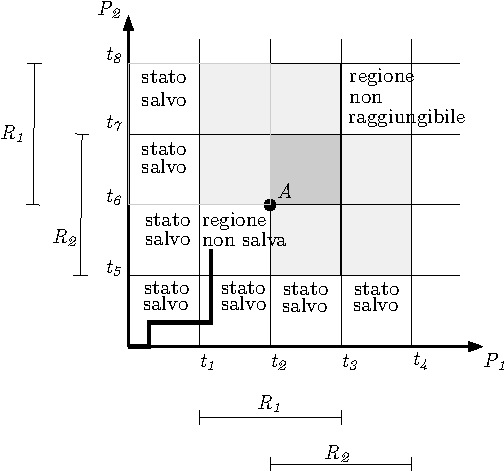
\includegraphics{img/sincronizzazione/matrice-stati-sicuri.pdf}
  \caption{Esempio di prevenzione dinamica per mezzo di matrice degli stati sicuri}
  \label{fig:matrice-stati-sicuri}
\end{figure}

Agli istanti $t_1$ e $t_2$ il processo $P_1$ richiede rispettivamente l'utilizzo
di $R_1$ e $R_2$, mentre a $t_3$ e $t_4$ tali risorse vengono rilasciate.
Analogamente fa $P_2$ con le medesime risorse agli istanti $t_5$, $t_6$
e $t_7$, $t_8$.
\\ \\
La traiettoria rappresenta il cammino di esecuzione dei due processi che
parte dall'origine e prosegue alternando l'esecuzione di $P_1$ e $P_2$.
Il punto \textit{A} rappresenta una situazione di blocco critico in quanto
corrisponde alla situazione in cui i due processi, possedendo ciascuno una risorsa,
chiedono di poter utilizzare l'altra, bloccandosi indefinitamente.
\\ \\
Scopo del sistema è fare in modo che la traiettoia di esecuzione proceda
attraversando sempre \emph{stati salvi} senza mai entrare in stati
\emph{non salvi}.
\\ \\
Nella Figura~\ref{fig:matrice-stati-sicuri}, qualunque sia il
proseguimento dell'esecuzione, il sistema è destinato a andare in
stallo.

\subsubsection{Individuazione di blocchi critici e recupero}
Sottosezione altrimenti nota come \emph{deadlock detection and recovery}.

\paragraph{Deadlock detection}
Periodicamente il sistema ricerca la presenza di condizioni sufficienti
allo stallo, analizzando eventuali cicli di dipendenze tra processi.

La ricerca di cicli in grafi è molto dispendiosa, pertanto questi
algoritmi vengono mandati in esecuzione raramente.

\paragraph{Deadlock recovery}
Esistono due tecniche:
\begin{itemize}
  \item terminazione forzata di tutti i processi del ciclo
  \item terminazione di un processo per volta finché non vengono
    liberate abbastanza risorse per permettere al sistema di ritornare
    a funzionare
\end{itemize}

\section{Gestione della memoria}

\subsection{Concetti generali}
Analogie con CPU:
\begin{itemize}
  \item risorsa necessaria implicitamente per un processo (non su
    richiesta)
  \item virtualizzazione
\end{itemize}

Differenze con CPU:
\begin{itemize}
  \item contesto del processo \emph{vs} area di swap
  \item la memoria può ospitare contemporaneamente più processi
    (richiede accortezze di protezione)
  \item opportunità di condivisione di tutta o parte della risorsa
\end{itemize}

\subsubsection{Terminologia utilizzata}
\begin{itemize}
  \item \textbf{funzione di rilocazione}, funzione $y = f(x)$ che
    traduce l'indirizzo virtuale $x$ nell'indirizzo fisico $y$;
  \item \textbf{MMU}, Memory Management Unit, dispositivo hardware atto
    alla traduzione di indirizzi, da virtuali a fisici, per mezzo di una
    apposita funzione di rilocazione;
  \item \textbf{swap-in}, \textbf{swap-out}, operazione di caricamento
    di un programma (o parte di esso) dalla memoria di massa verso la
    memoria centrale, e viceversa;
  \item \textbf{TLB}, Translation Lookaside Buffer, dispositivo hardware
    di caching associativo per velocizzare le operazioni più frequenti
    di traduzione di indirizzi, sfruttando i principi di località
    spaziale e temporale\footnote{Vedi \cite{frosini:architetturacalcolatori}}
\end{itemize}

\subsubsection{Caratteristiche della Gestione}
\begin{forest}
[ Caratteristiche della Gestione
  [ rilocazione
    [ statica ]
    [ dinamica ]
  ]
  [ memoria virtuale
    [ monolitica ]
    [ segmentata ]
  ]
  [ memoria fisica
    [ contigua ]
    [ non contigua ]
  ]
  [ caricamento
    [ unico ]
    [ on-demand ]
  ]
]
\end{forest}

\begin{itemize}
  \item Rilocazione
    \begin{itemize}
      \item Rilocazione statica: la traduzione degli indirizzi viene
        effettuata una sola volta all'atto del caricamento del programma
        da parte del caricatore (rilocante) nella memoria fisica;
        in caso di \emph{swap-out} e successivo \emph{swap-in}, il
        programma deve essere ricaricato nella stessa locazione fisica;
      \item Rilocazione dinamica: la traduzione degli indirizzi viene
        effettuata ogni volta che viene generato un indirizzo
        (virtuale), per mezzo di un apposito supporto hardware (MMU);
    \end{itemize}
  \item Organizzazione della memoria virtuale
    \begin{itemize}
      \item Memoria Virtuale Monolitica: lo spazio di indirizzamento
        virtuale di un programma viene organizzato come un unico blocco,
        in cui è possibile trovare le varie sezioni (logiche) di codice,
        dati e stack una di seguito all'altra (contigue);
      \item Memoria Virtuale Segmentata: lo spazio di indirizzamento
        virtuale di un programma viene logicamente diviso in più
        \emph{segmenti}, che rispecchiano la struttura immaginata dal
        programmatore (funzioni, strutture dati), alle quali è possibile
        assegnare diversi permessi (lettura, scrittura); più segmenti
        diversi possono così essere allocati in più regioni fisiche non
        contigue in qualunque ordine;
    \end{itemize}
  \item Organizzazione della memoria fisica
    \begin{itemize}
      \item Memoria Fisica Contigua: la sezione virtuale (o le singole
        sezioni virtuali) di un programma vengono caricate in memoria in
        modo contiguo;
      \item Memoria Fisica Non Contigua: blocchi virtuali di un
        programma, anche se contingui, possono essere caricati nella
        memoria fisica in pagine diverse in modo non contiguo;
    \end{itemize}
  \item Caricamento dei blocchi del programma
    \begin{itemize}
      \item Caricamento Unico: tutti i blocchi di un programma vengono
        caricati in memoria all'atto della creazione del processo, anche
        se alcuni potrebbero non essere mai utilizzati;
      \item Caricamento On-Demand: i blocchi di un programma vengono
        caricati in memoria a tempo di esecuzione di un processo, e solo
        se sono richiesti (in seguito a generazione di \emph{fault});
      \end{itemize}
\end{itemize}

Diverse combinazioni di queste modalità di rilocazione, caricamento e
organizzazione dello spazio fisico e virtuale danno luogo a diversi
schemi di gestione della memoria virtuale.

Delle 2\textsuperscript{4}~=~16 diverse potenziali combinazioni, alcune
sono impossibili, altre inutili o non significative, e sono riassunte
nella Figura~\ref{fig:mem:tecniche-grafo} e nella
Figura~\ref{fig:mem:tecniche-tabella}.

\begin{landscape}
\begin{figure}
\centering
\begin{forest}
[ Tecniche di gestione della memoria
  [ Rilocazione
    [ Allocazione, edge label={node[midway] {statica}}
      [ Spazio Virtuale, edge label={node[midway] {contiguo}}
        [ Caricamento, edge label={node[midway] {monolitico}}
          [ Partizioni fisse o variabili, edge label={node[midway] {unico}} ]
          [ Partizioni multiple, edge label={node[midway] {unico}} ]
        ]
      ]
    ]
    [ Allocazione, edge label={node[midway] {dinamica}}
      [ Spazio Virtuale, edge label={node[midway] {contiguo}}
        [ Caricamento, edge label={node[midway] {segmentato}}
          [ Segmentazione, edge label={node[midway] {unico}} ]
          [ Segmentazione a domanda, edge label={node[midway] {on demand}} ]
        ]
      ]
      [ Spazio Virtuale, edge label={node[midway] {non contiguo}} ]
        [ Caricamento, edge label={node[midway] {monolitico}}
          [ Paginazione, edge label={node[midway] {unico}} ]
          [ Paginazione a domanda, edge label={node[midway] {on demand}} ]
        ]
        [ Caricamento, edge label={node[midway] {segmentato}}
          [ Segmentazione con paginazione, edge label={node[midway] {on demand}} ]
        ]
    ]
  ]
]
\end{forest}
\caption{Combinazioni significative delle varie tecniche di gestione della memoria}
\label{fig:mem:tecniche-grafo}
\end{figure}
\end{landscape}

\begin{figure}[H]
\centering
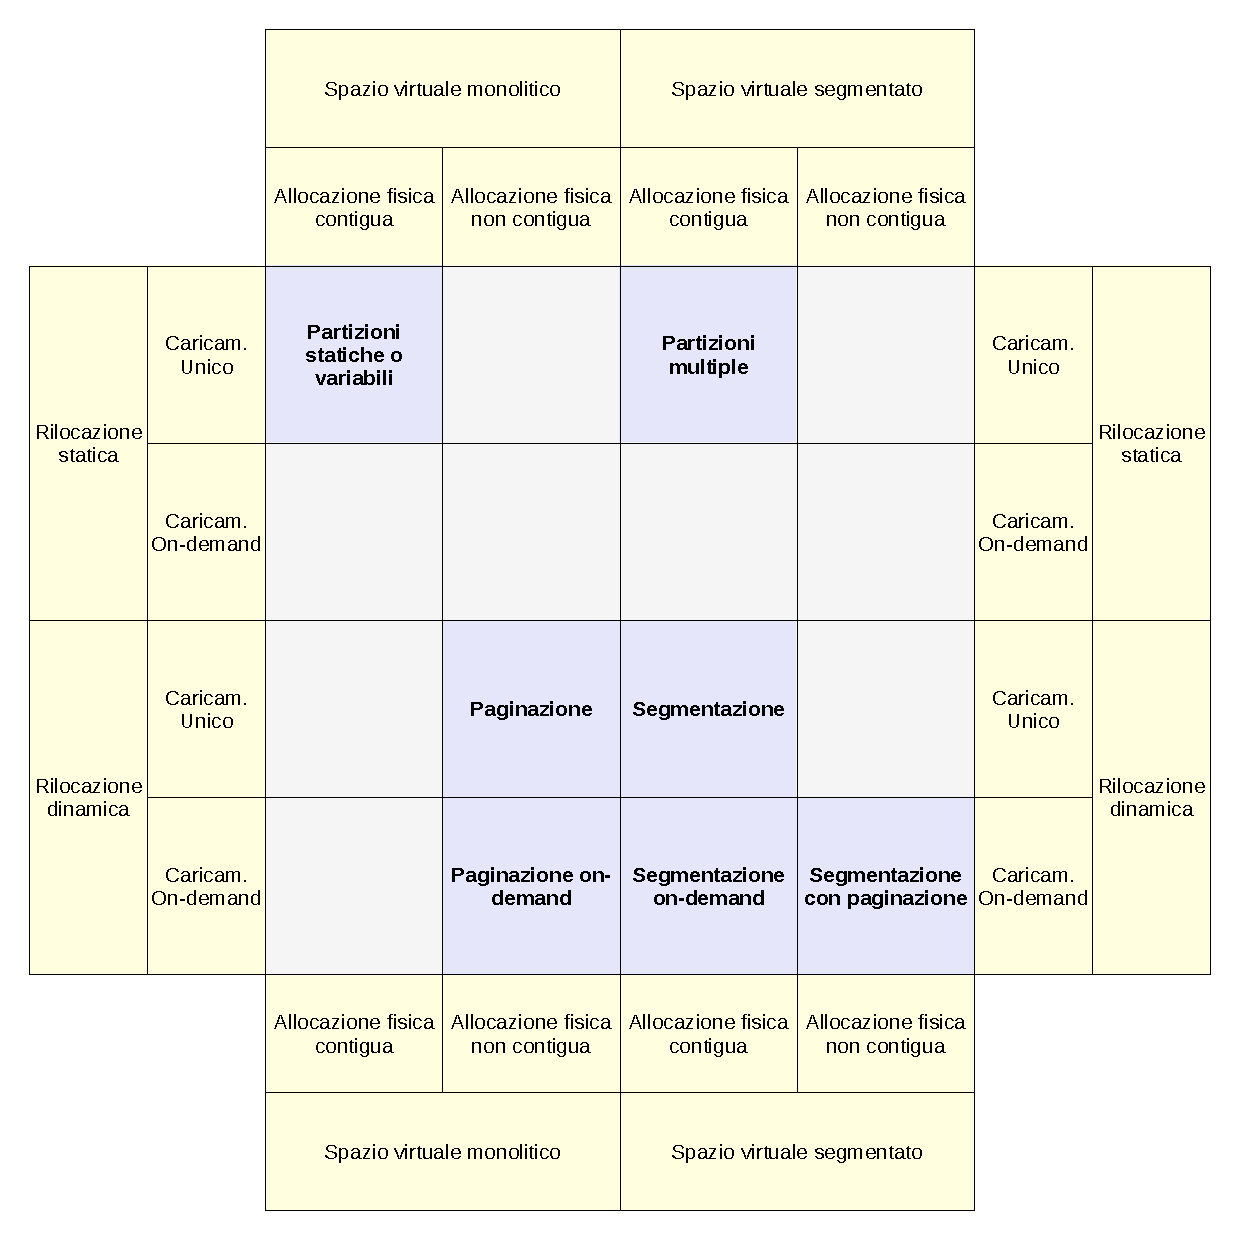
\includegraphics[width=16cm]{img/mem/TecnicheGestioneMemoria.pdf}
\caption{Combinazioni delle varie tecniche di gestione della memoria}
\label{fig:mem:tecniche-tabella}
\end{figure}

\subsection{Tecniche di gestione}
\begin{table}[H]
\begin{tabular}{| c | c | c | c | c |}\hline
  Tecnica                       & Rilocazione & Allocazione   & Spazio virtuale & Caricamento \\ \hline
  Partizioni fisse e variabili  & statica     & contigua      & monolitico      & unico       \\ \hline
  Partizioni multiple           & statica     & contigua      & segmentato      & unico       \\ \hline
  Segmentazione                 & dinamica    & contigua      & segmentato      & unico       \\ \hline
  Segmentazione on-demand       & dinamica    & contigua      & segmentato      & on-demand   \\ \hline
  Paginazione                   & dinamica    & non contigua  & monolitico      & unico       \\ \hline
  Paginazione on-demand         & dinamica    & non contigua  & monolitico      & on-demand   \\ \hline
  Segmentazione con paginazione & dinamica    & non contigua  & segmentato      & on-demand   \\ \hline
\end{tabular}
\end{table}

\subsection{Punti chiave delle varie tecniche}

\subsubsection{Partizioni fisse}
\begin{itemize}
  \item Frammentazione interna: per poter essere rilocato in una
    partizione, la dimensione di un programma in memoria deve essere
    minore (o al più uguale) alla dimensione della partizione in cui
    si intende rilocarlo. Ne consegue che spesso rimane dello spazio
    inutilizzato al termine della partizione, fenomeno che prende il
    nome di \emph{frammentazione interna}.
  \item Rotazione round robin: periodicamente il sistema operativo
    revoca la partizione della memoria di un processo e la assegna
    ad un altro, secondo la politica round robin.
\end{itemize}

\subsubsection{Partizioni variabili}
\begin{itemize}
  \item Frammentazione esterna: le partizioni variabili eliminano
    completamente il problema della frammentazione interna, ma
    introducono quello della \emph{frammentazione esterna}: quando
    un processo termina, infatti, la sua partizione di memoria
    torna disponibile, e lascia un "vuoto" tra partizioni occupate.
    Pur essendo la memoria totale "vuota" sufficiente a contenere
    l'immagine di un nuovo processo, la sua non contiguità rende
    praticamente impossibile il suo sfruttamento.
  \item Partizioni libere adiacenti: possono essere compattate in
    un'unica partizione libera più grande.
  \item Ricompattamento: lo spostamento fisico di tutte le
    partizioni al fine di ricompattare lo spazio occupato e quello
    libero è molto oneroso e, in questo caso particolare, non è
    applicabile in quanto trattasi di una tecnica con rilocazione
    statica.
  \item Lista: il sistema operativo mantiene una lista ordinata
    delle partizioni:
    \begin{itemize}
      \item schema \emph{best-fit}: lista ordinata per dimensione
        crescente delle partizioni: in fase di caricamento di un
        programma, la prima partizione libera di dimensione
        sufficiente a contenere il programma è anche quella che
        "calza meglio" (lo spazio che avanza prima della successiva
        partizione adiacente è minimo). In fase di scaricamento, la
        ricerca di partizioni adiacenti per il loro ricompattamento
        richiede però lo scorrimento di tutta la lista.
      \item schema \emph{first-fit}: lista ordinata per indirizzi
        crescenti delle partizioni: in fase di caricamento di un
        programma, la prima partizione libera di dimensione
        sufficiente a contenere il programma è quella che viene
        scelta, anche se non è quella che calza meglio. In fase di
        scaricamento, la ricerca di partizioni adiacenti è banale.
    \end{itemize}
\end{itemize}

\subsubsection{Segmentazione}
\begin{itemize}
  \item Segmenti: almeno tre segmenti, per codice, dati e stack,
    banalmente discernibili in hardware in stato di \emph{fetch},
    \texttt{ld}/\texttt{st}/\texttt{mov} e \texttt{push}/\texttt{pop}.
    Architetture più evolute prevedono la possibilità di utilizzare
    più segmenti, tramite la generazione di indirizzi del tipo
    \texttt{x = <segment, offset>} e la consultazione di una
    \emph{tabella dei segmenti}.
  \item Eccezioni:
    \begin{itemize}
      \item Protezione: segmento non appartenente al processo (errore);
      \item Protezione: offset al di fuori del segmento (errore o
        richiesta di allocazione);
      \item Protezione: flag R, W, X;
    \end{itemize}
  \item TLB: Translation Lookaside Buffer, cache associativa diventa
    necessaria per sopperire all'inefficienza del meccanismo.
  \item Condivisione: possibile, a condizione che segmenti
    semanticamente affini abbiano lo stesso numero;
\end{itemize}

\subsubsection{Segmentazione a domanda}
\begin{itemize}
  \item Presenza: flag P. Un segmento non presente genera
    un'eccezione di tipo \emph{segment fault}.
\end{itemize}
\begin{figure}[H]
\centering
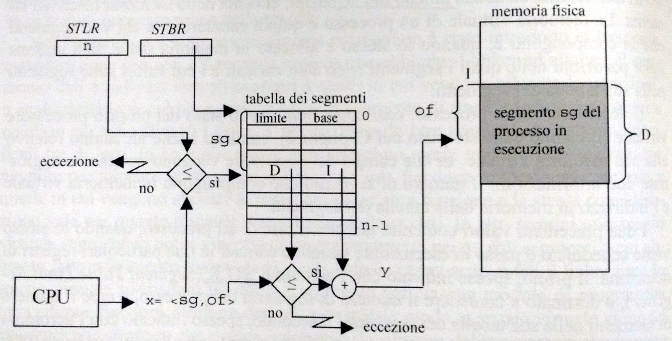
\includegraphics[width=10cm]{img/mem/trad-segmentazione.png}
\caption{Rilocazione dinamica nella segmentazione}
\end{figure}

\subsubsection{Paginazione}
\begin{itemize}
  \item Terminologia: \emph{pagina} o \emph{pagina virtuale}: regione
    in cui è diviso lo spazio virtuale; \emph{frame} o \emph{pagina
    fisica}: regione fisica in cui è divisa la memoria fisica;
    Le pagine sono mappate nei frame. Pagine consecutive non
    devono necessariamente essere mappate in frame consecutivi.
  \item Protezione: possibile ma meno significativa, in quanto la
    pagina, a differenza del segmento, riflette solo la struttura
    fisica della memoria e non la struttura semantica del programma;
  \item Pagine residenti: necessarie per trasferimenti DMA dall'IO
    o per funzioni vitali del sistema operativo;
  \item Trashing: situazione di funzionamento inefficace in cui le
    stesse pagine vengono continuamente swapped \emph{in} e
    \emph{out}.
  \item Condivisione: possibile, a condizione che gli indirizzi virtuali
    utilizzati da processi diversi uguali (puntatori).
\end{itemize}

\begin{figure}[H]
\centering
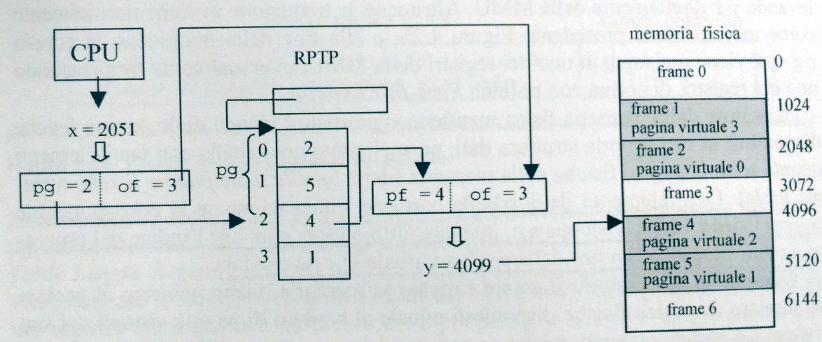
\includegraphics[width=10cm]{img/mem/trad-paginazione.png}
\caption{Rilocazione dinamica nella paginazione}
\end{figure}

\paragraph{Politiche di caricamento}
Alla creazione di un processo possono essere caricate le sue pagine:
\begin{itemize}
  \item tutte le pagine: ammesso di avere sufficiente memoria
    fisica a disposizione, in questo modo un fault può essere
    generato solo se il processo richiede l'allocazione di nuova
    memoria in maniera dinamica durante la sua esecuzione;
  \item alcune pagine: possono essere caricate solo le pagine
    indispensabili per l'"avvio" del processo, così le altre
    saranno caricate solo se questo ne fa richiesta;
  \item nessuna pagina: si fa affidamento solo sui fault, che
    verranno generati frequentemente nei primi istanti in cui
    il processo inizia ad essere eseguito;
\end{itemize}

\paragraph{Algoritmi di rimpiazzamento}
\begin{itemize}
  \item Ottimo: tengo un puntatore alla pagina che verrà
    utilizzata tra più tempo nel futuro (requisiti hardware:
    Mago Merlino veggente\footnote{https://www.youtube.com/watch?v=Icg6R5QWYwk});
  \item FIFO: i descrittori delle pagine fisiche frame sono organizzati
    in una lista circolare. Un puntatore punta sempre alla pagina
    fisica successiva all'ultima rimpiazzata, cioè alla pagina fisica
    successiva a quella più recente più recente, cioè alla pagina che è
    in memoria da più tempo.
  \item LRU, Least Recently Used: contrassegno ogni pagina fisica con il
    timestamp del suo ultimo accesso, e rimpiazzo la pagina che
    non viene usata da più tempo. Svantaggi: costoso in termini
    di tempo macchina e memoria, complesso da realizzare in
    hardware.
  \item Second Chance (orologio): l'MMU setta i bit di accesso
    (A, access) e modifica (D, dirty) alle pagine fisiche. Queste
    vengono organizzate in una lista circolare. Un puntatore punta
    sempre alla pagina successiva all'ultima rimpiazzata, cioè alla
    pagina che si trova in memoria da più tempo. In caso di
    rimpiazzamento, tuttavia, scorro la lista finché non giungo alla
    prima pagina fisica con A~=~0, ponendo il bit A~=~0 a tutte le
    pagine che incontro via via che scorro. Se tutte le pagine hanno il
    bit A~=~0, l'algoritmo rispecchia automaticamente l'algoritmo FIFO.
\end{itemize}

\paragraph{Tipi di rimpiazzamento}
\begin{itemize}
  \item Locale: le pagine vittime vengono scelte solo tra le pagine
    del processo che ha generato il page fault; ad ogni processo viene
    assegnato un \emph{budget} alla sua creazione, e le pagine gli
    vengono revocate se lo supera;
  \item Globale: le pagine vittime vengono scelte tra le pagine di
    tutti i processi;
\end{itemize}

\subsubsection{Segmentazione paginata}
\begin{figure}[H]
\centering
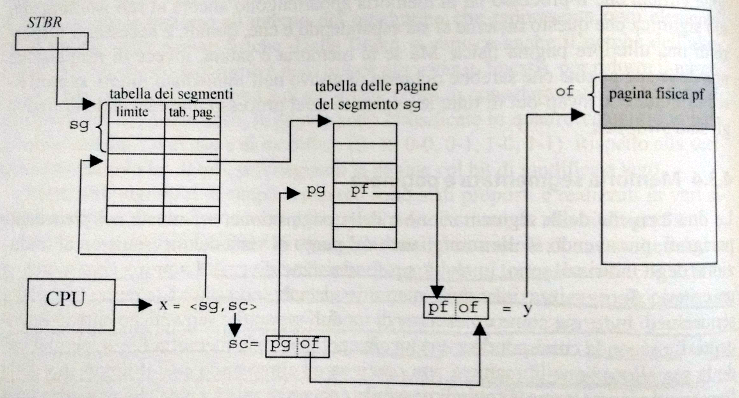
\includegraphics[width=10cm]{img/mem/trad-segmentazione-paginata.png}
\caption{Rilocazione dinamica nella segmentazione paginata}
\end{figure}

\subsection{Stati di un processo swapped}
\begin{figure}[H]
\centering
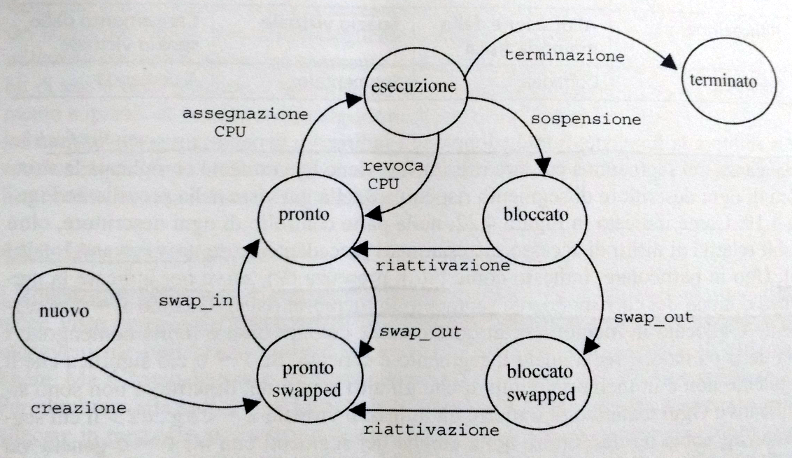
\includegraphics[width=10cm]{img/mem/stati-processo-swapped.png}
\caption{Stati di un processo swapped con caricamento unico}
\end{figure}

\section{Gestione I/O}

Questa sezione è fatta male. Studia il materiale dell'esame di Calcolatori Elettronici.

\begin{figure}[H]
\centering
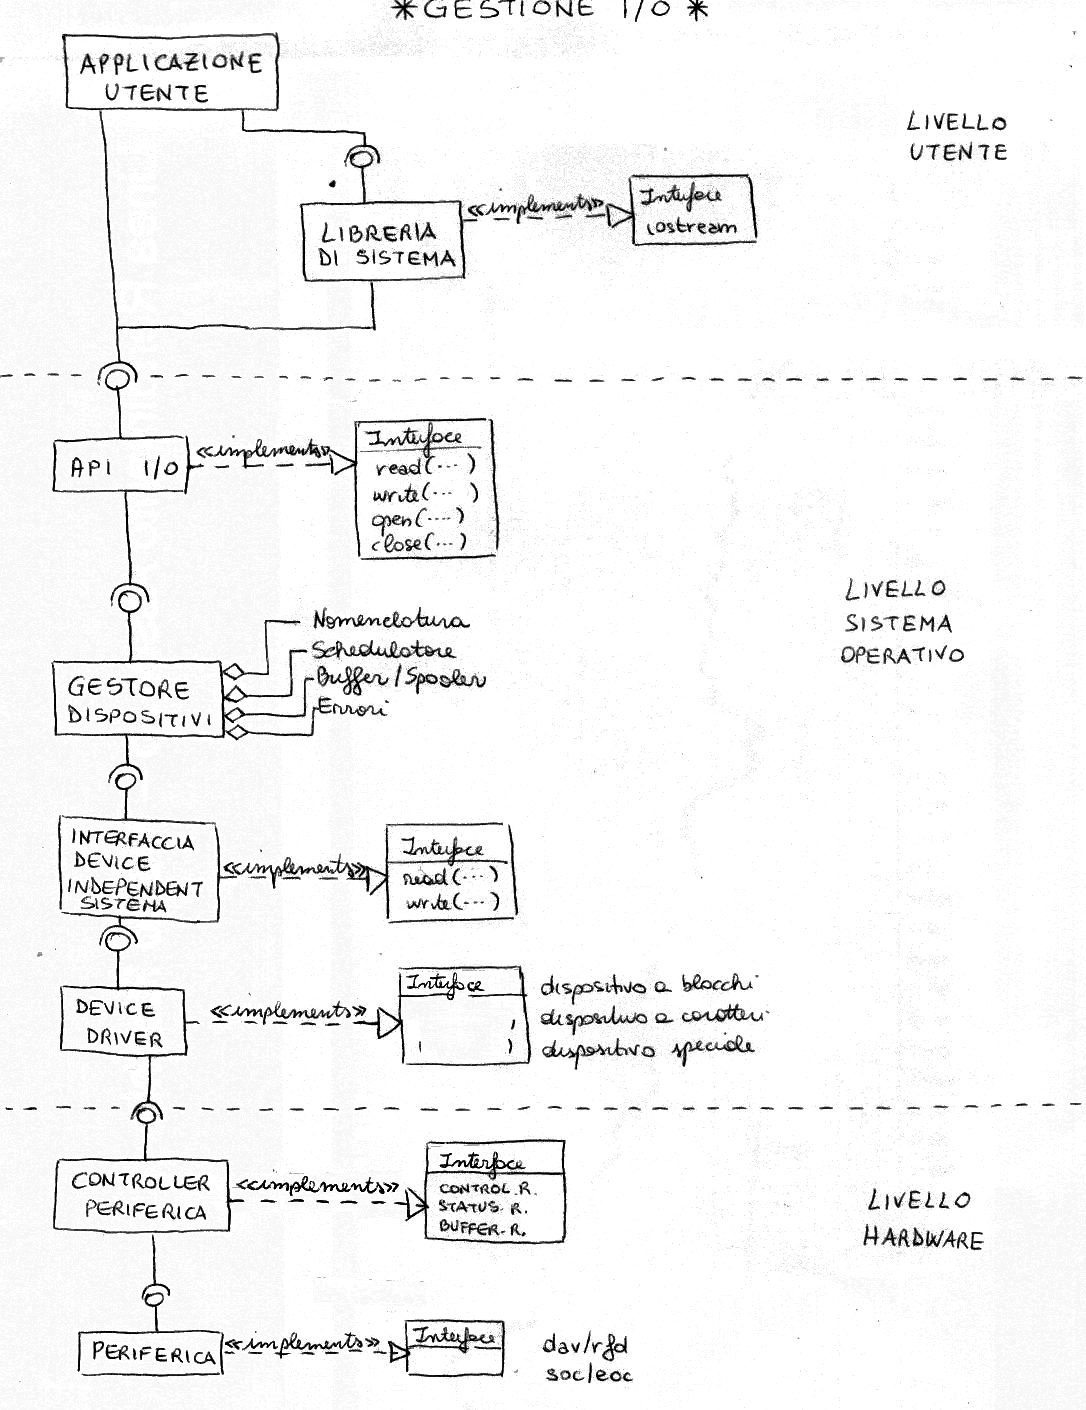
\includegraphics[width=17cm]{img/io/io-abstract.png}
\caption{Organizzazione logica del sottosistema di I/O tramite notazione approssimativa e inappropriata}
\end{figure}

Descrittore di un dispositivo:
\begin{verbatim}
  struct DescrittoreDispositivo {
    void* puntStatus;
    void* puntControl;
    void* puntData;
    semaforo datoDisponibile;
    char* buffer;
    int contatore;
    int esito;
  };
\end{verbatim}

\begin{figure}[H]
\centering
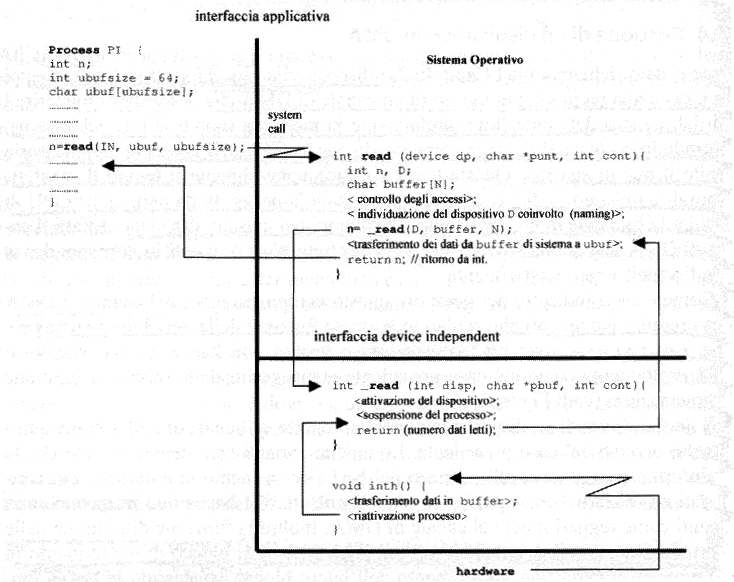
\includegraphics[width=18cm]{img/io/io-int.png}
\caption{Flusso di controllo durante l'esecuzione di una primitiva di I/O con interruzione}
\end{figure}

\begin{itemize}
\item Device independent
  \begin{itemize}
    \item Nomenclatura
    \item Protezione
    \item Buffering
    \begin{itemize}
      \item Buffer utente / sistema
      \item Sincronizzare produttore / consumatore
      \item Leggere meno dati del blocco
      \item Realizzare cache software
      \item Buffer di sistema residenti
    \end{itemize}
    \item Errori
    \begin{itemize}
      \item Errori recuperabili / Irrecuperabili
    \end{itemize}
    \item Allocazione dinamica dispositivi
    \item Spooling
  \end{itemize}
\end{itemize}

Seguono delle versioni molto approssimative di funzioni di gestione
dell'I/O: non c'è scritto quasi nulla, perché dipendono dal particolare
tipo di hardware, dal tipo di trasferimento (a interruzione o in DMA),
e da numerosi altri fattori.

System call read(), chiamata dall'applicazione:
\begin{verbatim}
  int read(file devicename, char* ubuffer, int n) {
    // Codice eseguito con privilegi di sistema
    ··· Controllo permessi di accesso al dispositivo `devicename` ···
    D = f(devicename); // Traduzione del nome
    ··· Garantisco mutua esclusione ···
    r = _read(D, sbuffer, n);
    memcpy(ubuffer, sbuffer, n);
    return r;
  }
\end{verbatim}

System call \_read(), chiamata dal sistema:
\begin{verbatim}
  int _read(int deviceid, char* sbuffer, int n) {
    descriptor[deviceid].buffer = sbuffer;
    descriptor[deviceid].count = n;
    ··· Abilito dispositivo a mandare interruzioni ···
    ··· Avvio il trasferimento dal dispositivo (bit start = 1) ···
    wait(descriptor[deviceid].eot);
    if (descriptor[deviceid].result == <tutto ok>) {
      return n - descriptor[deviceid].count;
    }
    else
      return -1;
  }
\end{verbatim}

Interrupt handler inth(), chiamato dal processo esterno:
\begin{verbatim}
  void inth() {
    ··· Disabilito dispositivo a mandare interruzioni ···
    c = get(descriptor[deviceid].addr_data);  // Leggo dato dal registro dati
    *descriptor[deviceid].buffer = c;
    ++descriptor[deviceid].buffer;
    if (--descriptor[deviceid].count == 0) {
      ··· Imposto descriptor[deviceid].result ···
      signal(descriptor[deviceid].eot);
    }
    else {
      ··· Riabilito dispositivo ···
    }
  }
\end{verbatim}

\subsection{Gestione timer}
Versione ibrida Calcolatori/Sistemi.

System call delay(), chiamata dall'applicazione:
\begin{verbatim}
  struct delay_s {  // Lista di delay_s
    int n;
    condition awake;
    struct delay_s* next;
  };

  int delay(int n) {
    +---+     +---+     +---+
    |   | --> |   | --> |   |
    +---+     +---+     +---+

    ··· ricerca di delay_s D tale che n == SUM_precedenti(delay_s.n) ···
    ··· se non esiste, creazione di D e inserimento ···

    D.awake.wait();
  }
\end{verbatim}

Interrupt handler inth(), chiamato dal processo esterno:
\begin{verbatim}
  void inth() {
    D = <lista>; // primo elemento
    if (--D.n == 0) {
      D.awake.signal_all();
      <lista> = D.next;
      free(D);
    }
  }
\end{verbatim}

\subsection{Gestione dischi}
\subsubsection{Terminologia utilizzata}
\begin{itemize}
  \item TF = TA + TT; tempo medio
  \item TA = TS + RL; tempo di accesso
  \item TS; tempo di seek
  \item RL; rotation latency
  \item TT; tempo di trasferimento del settore
\end{itemize}

\subsubsection{Schedulazione}
\begin{itemize}
  \item FCFS, First Come First Served, altamente inefficiente;
  \item SSTF, Shortest Seek Time First, molto efficiente, ma soffre di
    starvation;
  \item SCAN, scansione continua del disco dalla prima all'ultima traccia,
    miglior compromesso tra FCFS e SSTF, ha buone prestazioni e non
    soffre di starvation;
\end{itemize}

\section{File System}
\subsection{Stack di astrazione}
\begin{table}[H]
  \centering
  \begin{tabular}{| c |}\hline
  \emph{Applicazioni} \\ \hline
  Struttura logica \\ \hline
  Accesso \\ \hline
  Organizzazione fisica \\ \hline
  Dispositivo virtuale \\ \hline
  \emph{Hardware} \\ \hline
  \end{tabular}
  \caption{Stack di astrazione}
\end{table}

\subsection{Visione d'insieme}
\begin{forest} giombatree,
[ Filesystem
  [ Struttura logica
    [ File - descrittore ]
    [ Directory - descrittore ]
    [ Organizzazione logica
      [ albero ]
      [ grafo diretto aciclico ]
    ]
  ]
  [ Accesso
    [ Sequenziale ]
    [ Diretto / Casuale ]
    [ Indicizzato ]
  ]
  [ Allocazione
    [ Contigua ]
    [ Lista
      [ FAT ]
    ]
    [ Indice
      [ Indice a più livelli ]
    ]
  ]
]
\end{forest}

\subsubsection{Struttura logica}
Terminologia utilizzata:
\begin{itemize}
  \item \textbf{file}, sequenza di informazioni organizzate in record;
  \item \textbf{record}, unità logica minima di informazione all'interno
    di un file (es. \emph{linea}, \emph{byte}, ...);
\end{itemize}

Organizzazione del filesystem:
\begin{itemize}
  \item albero;
  \item grafo diretto aciclico;
\end{itemize}

Descrittore di file:
\begin{verbatim}
struct file_descriptor_s {
  string  nome;
  uint    dimensione;
  sector  indirizzo;
};
\end{verbatim}

Il descrittore può contenere anche altre informazioni di utilità, quali
il tipo, la data di creazione o di ultima modifica del file, e
informazioni di protezione, quali utente e gruppo proprietaro e
relativi permessi di accesso.

\subsubsection{Accesso}
I descrittori possono essere memorizzati:
\begin{itemize}
  \item nel file rappresentante la directory di appartenenza:
  \begin{itemize}
    \item il sistema è distribuito;
    \item il linking necessita di costosi
      barbatrucchi;\footnote{workaround, espedienti creativi}
  \end{itemize}
  \item in un'area dedicata del disco; la directory contiene i puntatori
    ai descrittori di file:
  \begin{itemize}
    \item il sistema è centralizzato in un'area dedicata del disco;
    \item il linking è banale;
  \end{itemize}
\end{itemize}

Il sistema può fornire una (o più) delle seguenti interfacce:
\begin{itemize}
  \item Accesso sequenziale: l'accesso al record \emph{i}-esimo
  richiede l'accesso a tutti i precedenti $ i - 1 $ record.
  \item Accesso diretto: l'accesso ai record avviene in modo
  indicizzato, numericamente, in modo analogo ad un vettore.
  \item Accesso indicizzato: l'accesso ai record avviene tramite
  l'associazione di un'etichetta al record; è necessaria una tabella
  associativa all'interno del file; questo approccio è tipico
  dei DBMS\footnote{Database Management System}.
\end{itemize}

\subsubsection{Organizzazione fisica}
Un dispositivo hardware viene astratto con un dispositivo
virtuale, ad es. un hard disk viene astratto come un insieme di blocchi
da 512 byte ciascuno, indicizzati dalla tupla
CHS\footnote{Cilinder Head Sector}.

\begin{table}[H]
\centering
\begin{tabular}{| p{8cm} | c |}\hline
  Allocazione contigua  & 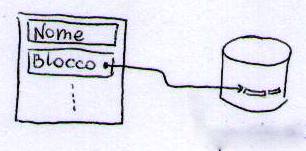
\includegraphics[width=5cm]{img/fs/alloc-contigua.png}  \\ \hline
  Allocazione a lista, eventualmente ridondata tramite FAT & 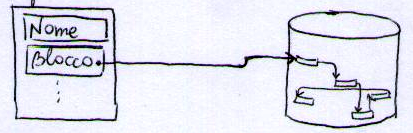
\includegraphics[width=5cm]{img/fs/alloc-lista.png}  \\ \hline
  Allocazione a indice, eventualmente a più livelli & 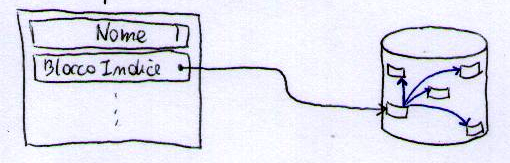
\includegraphics[width=5cm]{img/fs/alloc-indice.png}  \\ \hline
\end{tabular}
\caption{Tipi di allocazione fisica}
\end{table}

\paragraph{FAT, File Allocation Table}
Struttura ridondante per filesystem con allocazione fisica a lista:
la tabella contiene un'entrata per ogni settore del disco, che associa,
ad ogni settore, il suo successivo.

\section{Protezione}
\begin{itemize}
  \item \textbf{soggetto}: parte attiva di un sistema che accede a degli
    oggetti per conto degli utenti, es. processi;
  \begin{itemize}
    \item soggetto = (processo, dominio di protezione)
  \end{itemize}
  \item \textbf{oggetto}: parte passiva di un sistema, es. risorse
    fisiche o logiche;
\end{itemize}

Politiche di protezione:
\begin{itemize}
  \item \textbf{DAC}, Discretionary Access Control, i diritti di accesso
    agli oggetti vengono definiti dai loro proprietari;
  \item \textbf{RBAC}, Role-based Access Control, i diritti di accesso
    agli oggetti vengono definiti da un'entità amministratrice e vengono
    assegnati a gruppi di utenti che rappresentano degli specifici ruoli
    all'interno di una organizzazione;
  \item \textbf{MAC}, Mandatory Access Control, i diritti di accesso
    agli oggetti vengono definiti da un'entità amministratrice centrale,
    per esigenze di elevata sicurezza (militare, sanitaria);
\end{itemize}

Principio del minimo privilegio: a un soggetto vengono garantiti
i privilegi minimi indispensabili per lo svolgimento del suo compito.


\section{Unix}
\subsection{Unix puro}
\subsubsection{Generalità}
Sistema monolitico.

\subsubsection{Processi}
\begin{itemize}
  \item processi pesanti, no thread;
  \item spazio di indirizzamento dati privato;
  \item comunicazione tramite segnali;
  \item spazio di indirizzamento codice condiviso: il codice viene detto
    \emph{rientrante};
\end{itemize}

\begin{figure}[H]
  \centering
  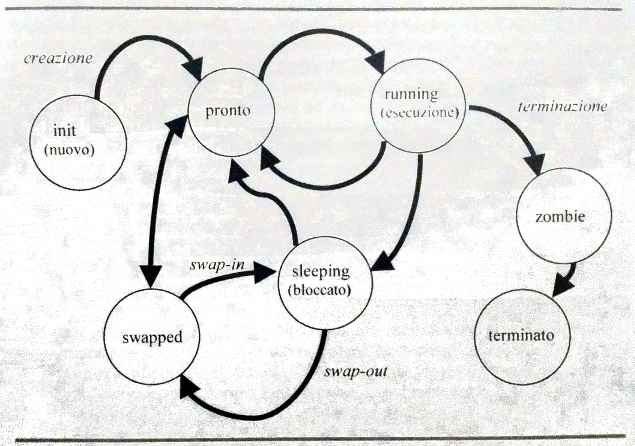
\includegraphics[width=7cm]{img/unix/stati-processo.png}
  \caption{Stati di un processo su Unix}
\end{figure}

Un processo diventa \emph{zombie} dopo che ha chiamato la \emph{system
call} di terminazione \texttt{exit()}, ma le sue strutture dati non
possono essere distrutte in quanto la sua immagine è
ancora necessaria: questo avviene sempre quando il processo
figlio intende terminare prima del processo padre, quest'ultimo non
è ancora terminato, e potrebbe quindi richiedere di conoscerne lo stato
di terminazione del figlio.

\paragraph{PCB, Process Control Block}\mbox{}\\
\begin{itemize}
  \item \textbf{Process Structure}, residente in memoria centrale,
    contiene informazioni vitali di cui il sistema deve sempre essere a
    conoscenza;
  \item \textbf{User Structure}, swappabile, contiene informazioni
    specifiche del processo che sono necessarie solo quando il processo
    è in esecuzione; può essere swappata quando il processo si trova
    nello stato swapped;
\end{itemize}

\begin{minipage}{1\linewidth}
\begin{minipage}{.45\linewidth}
Process Structure:
\begin{itemize}
  \item PID
  \item Stato
  \item Riferimento a area dati e stack
  \item Riferimento alla \emph{text structure}
  \item Parent PID
  \item Priorità
  \item Next process in coda
  \item Riferimento alla \emph{user structure}
\end{itemize}
\end{minipage}
\vline
\begin{minipage}{.45\linewidth}
User Structure:
\begin{itemize}
  \item Contesto registri generali CPU
  \item File allocati
  \item Segnali non ancora gestiti
  \item Proprietario, Gruppo
  \item Ambiente: cwd\footnote{Current Working Directory}, argc, argv
\end{itemize}
\end{minipage}
\end{minipage}

\paragraph{System call per la gestione dei processi}
\begin{itemize}
  \item int fork(void);
  \item int execl(char* path, char* arg0, char* arg1, ..., char* arg\textit{N}, (char*)0);
\end{itemize}

\paragraph{Schedulazione}
\begin{itemize}
  \item Priorità
    \begin{itemize}
      \item priorità $ \in [-20, +19] $;
      \item -20 è la priorità più alta, 19 quella più bassa;
      \item i processi utente hanno priorità positiva, i processi
        sistema hanno priorità negativa;
      \item un processo può diminuire volontariamente la sua priorità,
        ma non aumentarla; solo root può aumentare la priorità dei
        processi;\footnote{perché root è root, root è onnipotente, root
        può fare tutto, anche uccidere init\footnote{non lo fare!}}
    \end{itemize}
  \item Esiste una coda di processi per ogni livello di priorità;
  \item I processi dentro una singola coda sono gestiti \emph{round robin};
\end{itemize}

\subsubsection{Memoria}
Segmentazione paginata, on demand.

\subsubsection{Filesystem}
\begin{itemize}
  \item il descrittore di file viene detto \emph{inode};
  \item i descrittori sono memorizzati in una regione dedicata del disco
    detta \emph{inode-list};
  \item ogni descrittore è identificato da un \emph{inode-number};
  \item un record ha la dimensione di \emph{un} byte;
  \item le directory contengono puntatori agli inodes;
  \item allocazione dei file contigua/indirizzata 13-15 ?? TODO %% TODO %%
\end{itemize}

\subsection{Linux}
\subsubsection{Processi}
\begin{itemize}
  \item processi pesanti e threads;
\end{itemize}

\clearpage
\printbibliography[heading=bibintoc]

\end{document}
